\begin{circuitikz}[
    american, 
    >={Latex[length=2.5mm, width=1mm]},
    alt={A satellite image map of Egypt illustrating potential sources of geographical error in Eratosthenes measurement method. Red circular markers indicate the locations of Alexandria in the north near the Nile Delta and Syene further south along the Nile River. A thick black dashed line connects Alexandria and Syene, labeled as 5000 stadia. A vertical dashed line extends directly south from Alexandria, forming a 3 degree angular offset with the line leading to Syene. A green dashed line near the bottom highlights the Tropic of Cancer, showing a 1 degree vertical separation from the latitude of Syene.}
    ]

    \node[
        anchor=south west,
        inner sep=0
    ]
    (image)
    at (0,0)
    {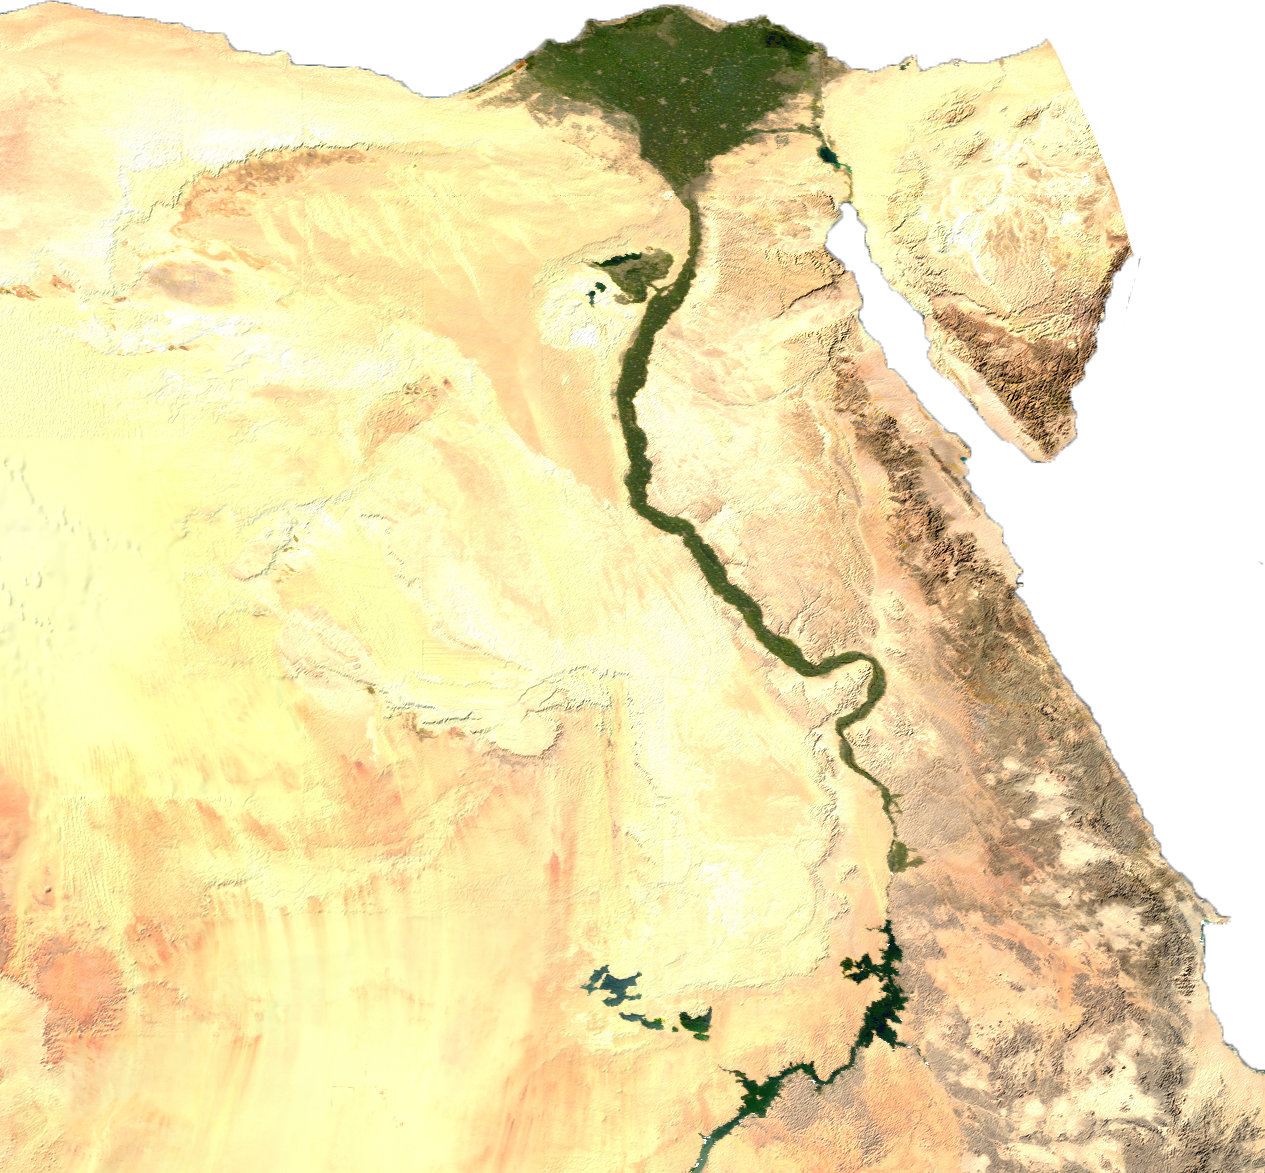
\includegraphics[width=10cm]{../../assets/images/Egypt_sat.png}};

    \begin{scope}[x={(image.south east)},y={(image.north west)}]
        \node[
            draw=BakerADARed, 
            fill=BakerADARed, 
            circle, 
            minimum size=0.5cm
        ] (alex)
        at (0.43,0.975) 
        {};
        
        \node[
            draw=BakerADARed, 
            fill=BakerADARed, 
            circle, 
            minimum size=0.5cm
        ] (syene)
        at (0.7,0.215) 
        {};

        \node[
            text=BakerBlack,
            draw=white,
            draw opacity=0.5,
            fill=white,
            fill opacity=0.5,
            text opacity=1,
            anchor=west,
            align=left
        ]
        at (alex.east)
        {Alexandria};

        \node[
            text=BakerBlack,
            draw=white,
            draw opacity=0.5,
            fill=white,
            fill opacity=0.5,
            text opacity=1,
            anchor=west,
            align=left
        ]
        at (syene.east)
        {Syene};

        \draw[
            BakerBlack,
            line width=3pt,
            dashed
        ]
        (alex.center)
        -- (syene.center)
        node[
            midway,
            right,
            draw=white,
            draw opacity=0.5,
            fill=white,
            fill opacity=0.5,
            text=BakerBlack,
            text opacity=1
        ]
        {5,000 stadia};

        \draw[
            BakerBlack,
            dashed
        ]
        (alex.center)
        -- (alex.center |- syene.center)
        coordinate(parallel);

        \draw[
            LakeBlue,
            line width=3pt
        ]
        (parallel)
        ++(0,0.2)
        arc[start angle=270, end angle=288, radius=0.609]
        node[
            midway,
            anchor=north west,
            draw=white,
            draw opacity=0.5,
            fill=white,
            fill opacity=0.5,
            text=BakerBlack,
            text opacity=1
        ]{$3^\circ$};

        \draw[
            UpNorthGreen,
            dashed,
            line width=3pt
        ]
        (0,0.1)
        -- (1,0.1)
        coordinate(cancer);

        \node[
            draw=white,
            draw opacity=0.5,
            fill=white,
            fill opacity=0.5,
            text=BakerBlack,
            text opacity=1,
            anchor=north east,            
        ]
        at (cancer)
        {Tropic of Cancer};

        \draw[
            BakerADARed,
            <->
        ]
        (cancer)
        -- (cancer |- syene.center)
        node[
            midway,
            right,
            text=BakerBlack
        ]{$1^\circ$};
    \end{scope}

\end{circuitikz}